% !Mode:: "TeX:UTF-8"

\chapter[基于图神经网络的语义依存图应用]{基于图神经网络的语义依存图应用}[Semantic Dependency Graph Application Based on Graph Neural Networks]

\section{引言}[Introduction]
\label{sec:chapter5-intro}

以句法依存树为代表的结构化信息,在传统的神经网络模型中被广泛应用于句子信息的获取。
例如,Socher等人\cite{socher-etal-2011-parsing}在2011年提出了递归神经网络,利用句法结构对文本进行编码。
随后在2015年,Tai等人在此基础上提出了Tree-LSTM,用于解决递归神经网络训练过程中的梯度消失和梯度爆炸问题。
随后一系列图神经网络\cite{kipf-welling-2017-semi, velickovic-etal-2018-gat}的提出,为自然语言处理领域的研究者提供了更多将句法等结构化信息融入神经网络模型中的选择。


自2018年以来,随着以BERT为代表的预训练模型在自然语言处理领域逐渐占据主流地位,其强大的表示和抽象能力使得结构化信息的作用开始受到质疑。
研究者开始设计方法对BERT中是否已经隐含句法等结构信息进行探测。
其中,Hewitt等人\cite{hewitt-manning-2019-structural}于2019年提出了计算BERT经过线性映射之后不同词之间距离的方法,并发现BERT中隐含有句中词在句法依存树上的距离信息。
而Jawahar等人\cite{jawahar-etal-2019-bert}和Lin等人\cite{lin-etal-2019-open}在同年发现,BERT的较低层的表示隐含更多句法信息,而较高层的的表示隐含更多语义信息。

尽管结构化信息在预训练时代的必要性受到了质疑,仍有一系列工作在尝试将句法树等结构化信息与预训练模型进行结合。
Fei等人\cite{fei-etal-2020-retrofitting}于2020年提出一种基于多任务学习的方法,在训练目标任务的同时预测句中词在句法树中的距离,隐式地将句法信息融入预训练模型中,从而提高了命名实体识别、情感分类、关系抽取等任务上的性能。
而Munir等人\cite{munir-etal-2021-adaptive}于2021年提出一种使用Tree-LSTM和CNN将句法信息融入BERT顶层输出的方法,并将其应用到语义角色标注任务上,取得了较好的结果。

在另一方面,由于图结构的语义表示是一个新兴课题,目前相关工作大部分都集中于语义图数据库的构建\cite{banarescu-etal-2013-abstract,abend-rappoport-2013-universal,oepen-etal-2015-semeval,che-etal-2016-semeval}和语义图分析方法的研究\cite{hershcovich-etal-2017-transition,dozat-manning-2018-simpler,cai-lam-2020-amr}。
在语义相关的结构化信息应用上目前仅有少量研究。
其中,Zhang等人\cite{zhang-etal-2020-semantics}于2020年提出将语义角色标注标签转化为表示向量,与从BERT中获取的表示向量合并,从而将语义角色标注信息融入BERT表示。
%他们将该方法应用于文本分类、自然语言推理和语义相似性任务上,并取得了明显的性能提升。
而Wu等人\cite{wu-etal-2021-infusing}于2021年提出使用图卷积网络\cite{kipf-welling-2017-semi}(Graph Convolutional Network,简称GCN)将语义依存信息融入BERT顶层输出中,并在文本分类、自然语言推理和语义相似性任务上验证了该方法的有效性。

现有的方法大部分都将预训练模型作为一个独立的词表示抽取器,仅仅使用它们获得词的表示向量,然后再使用与传统神经网络模型中相似的方法将结构化信息融入表示,并没有将结构化信息与预训练模型很好地结合。
此外,与大部分其他语言的预训练模型使用词片段作为基本输入单位不同,中文的预训练模型多使用字作为基本输入单位。
而由于此前方法首先用预训练模型获取词向量,然后在词向量基础上加入词级别的结构信息,在中文中很重要的字级别结构信息就被忽略了。

为了解决上述两个问题,本章提出基于字级别依存关系的强化预训练模型,首先将传统的词级别依存关系转化为字级别,然后利用图神经网络将这些结构融入预训练模型的每一层,从而将结构信息与预训练模型紧密结合在一起,获取了结构信息强化的预训练模型。
为了验证该方法的有效性,本章首先在中文语义角色标注任务上进行了实验,分别尝试将句法依存树信息和语义依存图信息融入预训练模型中,从而提高模型在该任务上的性能。
实验结果表明这两类信息都能有效提高模型性能,且建模的是不同类型信息,二者结合在一起时能进一步提高模型性能。
另外,本章还在中文关系抽取任务上进行了实验,进一步证明了语义依存图信息的融入对于模型性能提高的帮助。
本章提出的模型在这两个任务上都取得了目前最好结果。


\section{背景与相关工作}[Related Work]

语义角色标注任务于2000年被Gildea等人最先提出,在此后的二十年中,研究者一直致力于使用结构化的句法信息帮助该任务,并取得了显著效果。
而这些研究中的宝贵经验,对于实现本文的利用语义依存图信息帮助其他任务的目标具有很强的借鉴意义。
因此,本节首先介绍语义角色标注领域发展过程中结构化句法信息应用方法的演变,然后具体介绍其中近年来较常用的使用图卷积网络将结构信息融入神经网络模型的方法。

在语义角色标注研究的早期阶段,研究者普遍采用基于特征工程的方法\cite{zhao-etal-2009-multilingual-dependency,bjorkelund-etal-2009-multilingual,li-etal-2009-improving}。
在这一阶段,句法信息一般被用作额外的特征用于增强模型\cite{pradhan-etal-2005-semantic-role,che-etal-2006-hybrid}。
此后,随着神经网络模型在自然语言处理领域的广泛应用,该领域涌现出了一批不使用句法信息的(syntax-agnostic)基于神经网络的语义角色标注模型,获取了比使用句法信息的(syntax-aware)特征工程方法更好的结果。
其中,Fitzgerald等人\cite{fitzgerald-etal-2015-semantic}在2015年提出使用神经网络同时对论元及其标签进行建模。
Zhou等人\cite{zhou-xu-2015-end}于2015年将双向LSTM应用到基于词组的(span-based)语义角色标注中并取得了较好结果。
类似地,Marcheggiani等人\cite{marcheggiani-etal-2017-simple}将双向LSTM应用到基于词的(word-based)语义角色标注中并提升了其性能。
随着这些模型的提出,研究者开始讨论在深度学习时代句法信息是否还对语义角色标注有帮助。
而这种讨论又引出了一系列在神经网络框架下利用句法信息帮助语义角色标注的工作。
其中,Roth等人\cite{roth-lapata-2016-neural}在2016年提出了将句法树上的路径转化为向量向神经网络模型中加入句法信息的方法。
在2017年,Marcheggiani等人\cite{marcheggiani-titov-2017-encoding}和Qian等人\cite{qian-etal-2017-syntax}分别提出了使用图卷积网络和树结构LSTM对句法信息直接建模的方法。
沿着他们的脚步,Li等人\cite{li-etal-2018-unified}于2018年尝试了多种将句法信息融入神经网络模型的方法。
而Munir等人\cite{munir-etal-2021-adaptive}于2021年提出使用适应性卷积网络(adaptive convolution network)和Tree-LSTM将句法信息直接融入神经网络。

除了上述显式地将句法信息融入神经网络的工作外,还有一批工作尝试使用其他方式利用句法信息帮助语义角色标注。
例如,He等人\cite{he-etal-2018-syntax,he-etal-2019-syntax}尝试使用句法信息帮助模型进行论元剪枝,删除不可能的论元从而提高预测准确率。
Strubell等人\cite{strubell-etal-2018-linguistically}和Xia等人\cite{xia-etal-2019-syntax}分别提出了使用多任务学习框架同时学习句法分析任务和语义角色标注,从而隐式地将句法信息通过共享的参数传递给语义角色标注任务。

近年来,随着BERT等预训练模型在自然语言处理各领域取得重大成功,语义角色标注领域也出现了使用预训练模型的工作。
例如,Shi等人\cite{shi-lin-2019-simple}在BERT输出的基础上使用一个简单的序列标注框架用于解决语义角色标注任务,取得了显著优于此前最好结果的性能,为预训练时代的语义角色标注提供了一个很好的基线模型。
此后,Li等人\cite{li-etal-2020-high}在预训练模型的基础上将高维图结构特征引入模型中,进一步提高了模型性能。
与此同时,在预训练时代,结构化句法信息对于语义角色标注任务的帮助又受到了质疑。
正如第\ref{sec:chapter5-intro}节中介绍的,一系列针对BERT的探测任务表明其中已经隐含了结构化句法信息。
另一方面,在此前的使用句法信息的语义角色标注工作中,也有研究者发现当使用BERT代替传统上下文无关词向量作为模型输入时,加入句法信息带来的性能提升变得十分有限\cite{xia-etal-2019-syntax}。
这种发现也说明将结构化信息与预训练模型融合是十分具有挑战性的工作。

除了Marcheggiani等人使用图卷积网络利用句法信息帮助语义角色标注任务外,Wu等人\cite{wu-etal-2021-infusing}也于2021年使用图卷积网络将语义依存信息融入BERT模型,并应用于文本分类和自然语言推理等任务。
因此本节接下来对图卷积网络进行介绍。
具体来说,给定输入序列$w_1,w_2,\dots,w_n$,其中$w_v$在图卷积网络第$k+1$层的隐层状态为:
\begin{equation}
    \bm{h}_v^{(k+1)} = \text{ReLU}(\sum_{u\in \mathcal{N}(v)}\bm{W}^{(k)}\bm{h}_u^{(k)}+\bm{b}^{(k)})
\end{equation}
其中$\mathcal{N}(v)$表示词$w_v$在依存结构中的相邻节点,$\bm{h}_u^{(0)}$为词$w_u$的输入表示向量,ReLU为激活函数。
上述图卷积网络实现了依存结构中相邻节点之间的信息传递,当$N$层图卷积网络堆叠起来时,就实现了在依存结构中距离为$N$以内的节点间传递信息。

纵观语义角色标注领域的发展史,可以发现其对结构化句法信息的使用呈螺旋上升态势,即在每个新的时代开始时,随着更强模型的提出,句法信息的有效性就会受到质疑。
但之后随着新的建模结构化信息的方法的提出,又会证明句法信息仍然能有效地帮助语义角色标注。
因此本章以使用语义依存图帮助其他任务为目标,致力于解决结构化信息和预训练模型的融合问题。
本章针对中文预训练模型以字为基本输入单位的特点,提出了基于字级别依存关系的强化预训练模型,并在中文语义角色标注和关系抽取任务上验证了其有效性。


\section{基于字级别依存关系的强化预训练模型}[Pre-trained Model Enhancement Based on Character-Level Dependency Relations]

\subsection{预训练模型的基本输入单元}[Basic Input Units in Pre-trained Models]

本文第\ref{sec:chapter1-informal}节中已对预训练模型BERT进行了介绍。
其使用遮盖语言模型作为学习目标,将目标词遮盖后利用其上下文预测该词,实现了同时利用左右两个方向的上下文信息。
以BERT为代表的预训练模型的一个重要特点是词片段(word piece)向量\cite{wu-etal-2016-google}的使用。
这些词片段向量代替了传统神经网络模型中的词向量,成为了英文等很多语言中预训练模型的基本输入单元。
例如,在英文BERT中,词“devising”将被切分成“de”,“\#\#vis”和“\#\#ing”三个词片段(其中“\#\#”表示该词片段不是词中的第一部分),然后这些词片段的向量将被当做BERT模型的输入。
一般认为词片段的引入,能够有效缓解神经网络模型中的未登录词问题。
然而,在实际应用中,英文BERT的词表中仍然包含大量整词,只有一少部分词在英文BERT中被切分为了词片段。

\begin{figure}[hbtp]
	\centering
	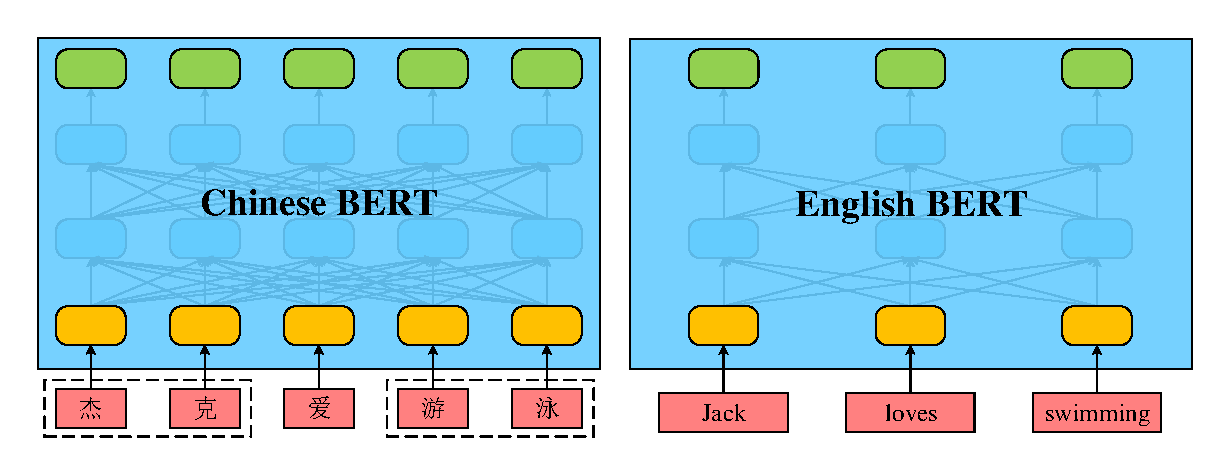
\includegraphics[width=0.98\textwidth]{figures/zh-vs-en-bert.pdf}
	\bicaption[fig:zh-vs-en-bert]{}{中文BERT(左)与英文BERT(右)对比示意图}{Fig.$\!$}{Comparison between Chinese BERT (left) and English BERT (right).}
\end{figure}

与其他大部分语言不同的是,在中文上,以BERT为代表的预训练模型往往使用字而不是词片段作为基本输入单元。
而由于中文中很大一部分词都是由超过一个字组成的,在中文预训练模型中,一个词由多个基本单元组成的现象十分常见。
图\ref{fig:zh-vs-en-bert}给出了中文BERT与英文BERT的对比示意图,对于句子“杰克爱游泳”(“Jack loves swimming”),在中文BERT上三个词中有两个词都被切分成了基本输入单元字,而在英文BERT上,三个词都没有被切分成词片段。

为了进一步证明这一点,本节在CoNLL 2009\cite{hajic-etal-2009-conll}多语言语义角色标注数据集上统计了各个语言的训练集中多基本单元词(由多个基本输入单元组成的词)所占的比例,结果如表\ref{tbl:multi-unit-word}所示。
结果表明,中文上的多基本单元词所占的比例超过了总词数的一般,要远高于其它语言。
在其他语言中,多基本单元词比例最高的德语中也仅有21\%的词由多个基本输入单元组成。
该发现充分说明了在中文预训练模型中,作为基本输入单元的字之间的关系的重要性。
因此,本章提出基于字级别依存关系的强化预训练模型,将这种重要的字间关系融入预训练模型中,从而增强其表示能力。

\begin{table}[htpb]
    \bicaption[tbl:multi-unit-word]{}{CoNLL 2009各语言训练集数据}{Table$\!$}{Training set statistics of different languages in CoNLL 2009.}
    \vspace{0.5em}\centering\wuhao
    \begin{tabular}{lccc}
        \toprule[1.5pt]
        语言 & 句子数 & 词数 & 多基本单元词比例\%  \\
        \midrule[1pt]
        中文  & 22,277  & 609,060  & 53.21 \\
        英文  & 39,279  & 958,167  & 14.37 \\
        德语   & 36,020  & 648,677  & 21.00 \\
        西班牙语 & 14,329  & 427,442  & 12.45 \\
        \bottomrule[1.5pt]
    \end{tabular}
\end{table}

最近,El Boukkouri等人\cite{el-boukkouri-etal-2020-characterbert}提出了一个基于字母的英文BERT,与基于词片段的英文BERT相比,其中可能存在更多的多基本单元。
他们仅仅在英文上训练了这种基于字母的BERT,而对于其他很多语言,现有的预训练模型基本都还是基于词片段的。
此外,由于本文的主要研究内容是中文语义依存图的应用,且目前自然语言处理领域绝大部分研究者仍然在英文等其他语言上使用基于词片段的预训练模型,而在中文上使用基于字的预训练模型,本章将集中研究中文的预训练模型和依存结构和融合方法。

\subsection{字级别依存关系强化网络}[Character-Level Dependency-Infused Network]
\label{sec:chapter5-char-level-dep-infusion}

\begin{figure}[hbtp]
	\centering
	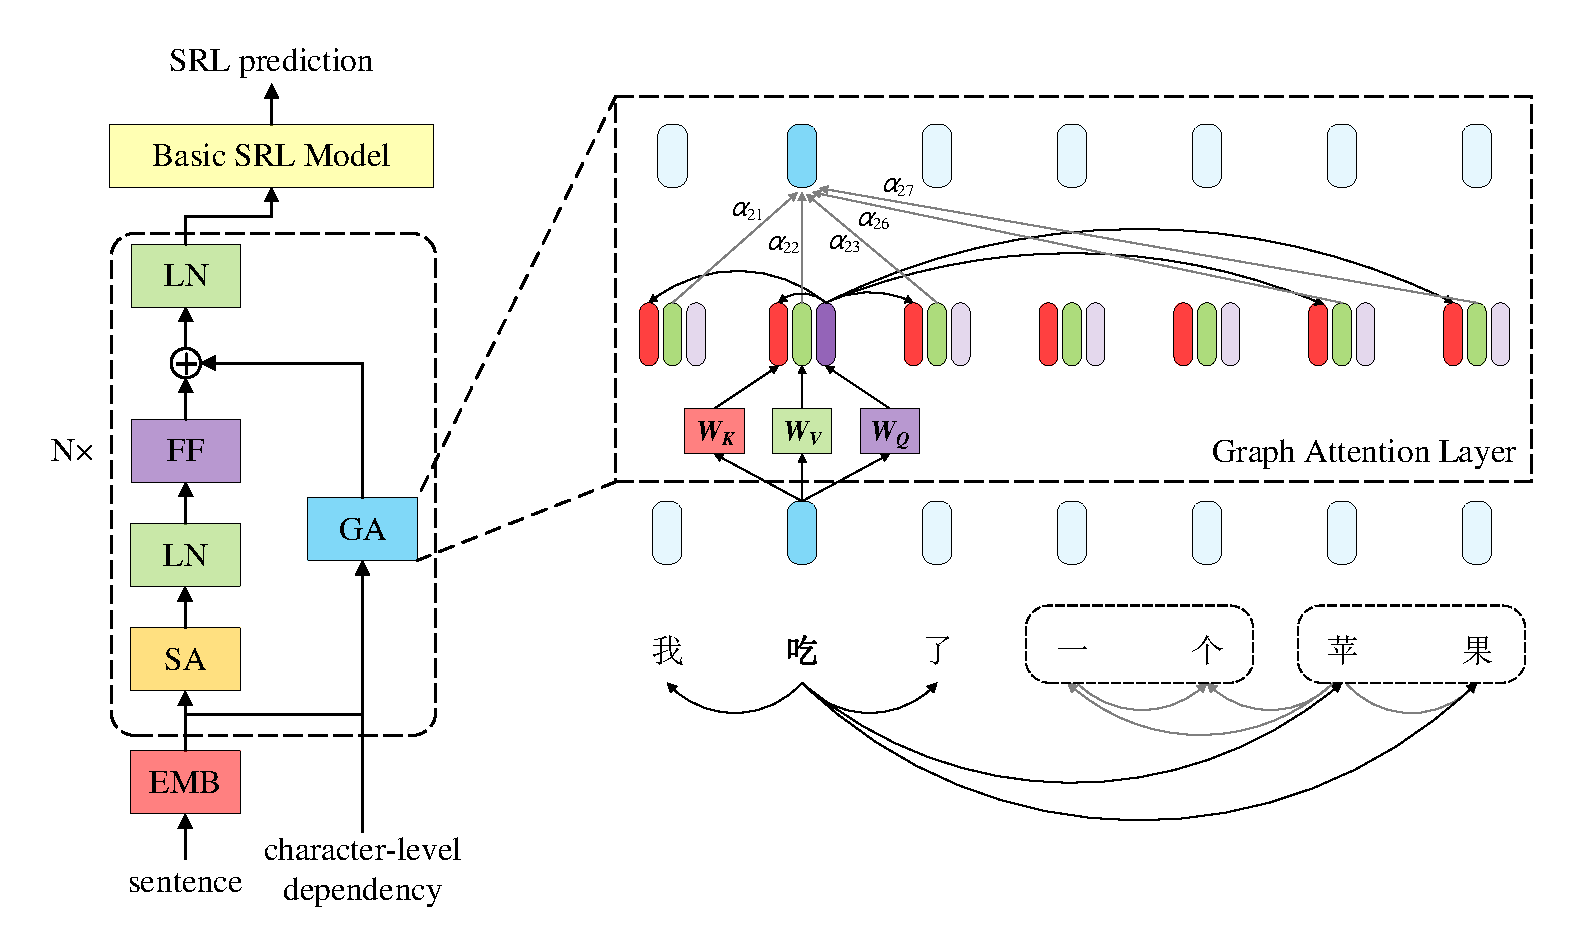
\includegraphics[width=0.95\textwidth]{figures/dependency-infused-network.pdf}
	\bicaption[fig:dependency-infused-network]{}{字级别依存关系强化网络结构示意图}{Fig.$\!$}{Character-Level Dependency-Infused Network.}
\end{figure}

本节将具体介绍本章提出的字级别依存关系强化网络,其结构如图\ref{fig:dependency-infused-network}所示。
该模型建立在中文BERT模型的基础上,图中EMB表示输入字向量(embeddings),SA表示自注意力层(self-attention layer),LN表示层标准化(layer normalization),FF表示前馈层(feed-forward layer),而GA表示图注意力层(graph attention layer)。

图注意力网络\cite{velickovic-etal-2018-gat}(Graph Attention Network,简称GAT)是自注意力网络的一种变体,通过注意机制将图结构融入神经网络中,模型中的图注意力层使用图注意力网络将字级别依存关系融入到预训练模型每一层。
具体来说,假设$\bm{h}_i$表示输入第$i$个字的隐层状态,图注意力网络首先计算各个字之间的相关分数:
\begin{equation}
    \label{eq:inter-score}
    s_{ij} = (\bm{h}_i\bm{W}_Q)(\bm{h}_j\bm{W}_K)^{\top}
\end{equation}
其中$\bm{h}_i\bm{W}_Q$和$\bm{h}_j\bm{W}_K$分别被称为查询(query)向量和键(key)向量,它们的乘积表示第$i$个字和第$j$个字之间的相关分数。
之后,该网络使用上述分数计算注意力分数:
\begin{equation}
\label{eq:att-score}
	\alpha_{ij} =\frac{\exp(s_{ij})}{\sum_{k\in\mathcal{N}_i}\exp(s_{ik})}
\end{equation}
其中$\mathcal{N}_i$表示第$i$个字在依存图中的邻居节点。
最后,第$i$个字经过依存图强化的输出为:
\begin{equation}
    \label{eq:gat-output}
	\bm{g}_i =\sum_{j\in \mathcal{N}_i}\alpha_{ij}(\bm{h}_j\bm{W}_V)
\end{equation}
其中$\bm{h}_j\bm{W}_V$称为值(value)向量。
假设将所有输入字的隐层状态拼接起来表示为$\bm{H} = [\bm{h}_1;\bm{h}_2; \dots; \bm{h}_n]$,而图注意力层输出的每个字的表示拼接起来表示为$\bm{G} = [\bm{g}_1;\bm{g}_2; \dots; \bm{g}_n]$,则上述图注意力层记为$\bm{G} = \text{GA}(\bm{H})$。

对于整个模型来说,其第$n$层的隐层状态$\bm{H}^n$通过如下方式计算:
\begin{equation}
	\label{eq:multi-att}
	\bm{A}^n = \text{LN}(\text{MultiAttn}(\bm{H}^{n-1}) + \bm{H}^{n-1})
\end{equation}
\begin{equation}
	\label{eq:ff}
	\bm{H}^n = \text{LN}(\text{FF}(\bm{A}^{n}) + \bm{A}^{n} + \text{GA}(\bm{H}^{n-1}))
\end{equation}
其中LN表示层标准化,$\bm{H}^0$表示输入字向量,而最高层隐层表示$\bm{H}^N$作为该模型输出的包含字级别依存信息的字表示,被输入其他任务的模型。
其中MultiAttn表示多头自注意力层,是由多个自注意力网络(SA)拼接而成,每个自注意力网络计算方式与公式\ref{eq:inter-score},\ref{eq:att-score}和\ref{eq:gat-output}中的图注意力网络计算方式基本相同,只是在计算最终输出时要考虑当前字与所有字而不是只与其相邻字之间的关系,需要将公式\ref{eq:gat-output}变为:
\begin{equation}
    \label{eq:sa-output}
	\bm{h}_i =\sum_{j=1}^{n}\alpha_{ij}(\bm{h}_j\bm{W}_V)
\end{equation}
另外公式\ref{eq:ff}中的FF表示前馈层:
\begin{equation}
    \text{FF}(\bm{h}) = \text{GELU}(\bm{W}\bm{h} + \bm{b})
\end{equation}
其中GELU为激活函数。

\subsection{字级别依存关系构建}[Construction of Character-Level Dependencies]

第\ref{sec:chapter5-char-level-dep-infusion}节中介绍的字级别依存关系强化网络需要输入序列的字级别依存关系作为额外信息输入,但目前词级别依存关系标注无论在句法还是语义任务上都占据主流,因此接下来首要的问题是如何在现有的词级别依存关系基础上构建字级别依存图。

具体的,给定输入句子$X = \{w_1, w_2, \dots, w_n\}$,其中$w_i$表示第$i$个词,该句子的词级别依存结构(句法依存树或语义依存图)为$G_w(X)$。
$w_i \rightarrow w_j \in G_w(X)$表示$G_w(X)$中存在一条从$w_i$指向$w_j$的弧。
假设一个词$w_i$中包括$m$个字,即$w_i=\{c_{i1}, c_{i2}, \dots, c_{im}\}$。
首先生成词内弧(intra-word arcs),即包含每个词内各个字之间依存关系的弧。
将每个词中的第一个字视为其中心节点,然后加入由第一个字指向后面所有字的弧。
具体来说,对于词$w_i$,向字级别依存图$G_c(X)$中加入第一个词$c_{i1}$指向后面每个字$c_{i2}, \dots, c_{im}$的弧,即$c_{i1} \rightarrow c_{i2} \in G_c(X), \dots, c_{i1} \rightarrow c_{im} \in G_c(X)$。

接下来生成词间弧(inter-word arcs),即包含各词之间依存关系的弧。
对于$G_w(X)$中的弧$w_i \rightarrow w_j \in G_w(X)$,向字级别依存图$G_c(X)$中加入由其中的父节点$w_i$的第一个字$c_{i1}$指向其中的子节点$w_j$中的每一个字$c_{j1}, \dots, c_{jm}$的弧。
记为$c_{i1} \rightarrow c_{j1} \in G_c(X), \dots, c_{i1} \rightarrow c_{jm} \in G_c(X)$。

\begin{figure}[hbtp]
	\centering
	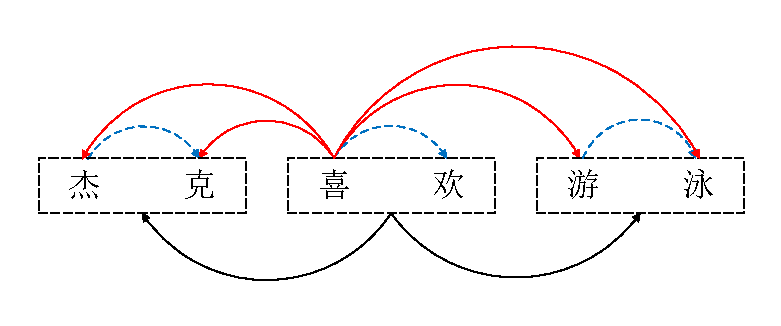
\includegraphics[width=0.75\textwidth]{figures/word-to-char.pdf}
	\bicaption[fig:word-to-char]{}{词级别(下)与字级别(上)依存关系转换示意图}{Fig.$\!$}{Converting word-level (lower) dependencies to character-level (upper).}
\end{figure}

图\ref{fig:word-to-char}中给出了从词级别依存关系转换为字级别依存关系的示意图,其中下方表示原始的词级别依存弧,上方红色实线表示字级别词间弧,蓝色虚线表示字级别词内弧。
由于在生成两种字级别依存弧的时候本章都选取了每个词的第一个字作为核心节点,每个词内的各个字的信息也通过词内弧传递到了第一个字,因此最终输出时使用每个词第一个字的隐层状态作为整个词的表示向量。


\section{字级别依存关系强化的预训练模型的应用}[Application of Character-Level Dependency-Enhanced Pre-trained Models]

本章第\ref{sec:chapter5-char-level-dep-infusion}节中介绍的字级别依存关系强化网络能有效将依存结构(句法依存树或语义依存图)融入预训练模型,从而获取结构信息强化的上下文相关词表示。
在此基础上,只需要使用前馈网络和softmax分类器等简单的神经网络模块就能完成很多自然语言处理任务,并有效提高预训练模型的性能。
本节将分别对基于强化预训练模型的命名实体识别和关系抽取模型进行介绍。

\subsection{基于预训练模型的命名实体识别模型}[Semantic Role Labeling Model Based on Pre-trained Models]

根据语义角色定义的不同,语义角色标注(Semantic Role Labeling,简称SRL)任务可以分为两类,即基于段的(span-based)语义角色标注和基于词的(word-based)语义角色标注。
其中前者使用多个连续的词组成的段作为语义角色,而后者则使用单个词作为语义角色。
本节选择基于词的语义角色标注作为目标任务,并使用CoNLL 2009\cite{hajic-etal-2009-conll}语义角色标注公开评测中的中文部分进行实验。

\begin{figure}[htbp]
	\centering
	\begin{dependency}[arc edge, arc angle=80, text only label, label style={above}]
	    \tikzstyle{label}=[draw=black, text=black, fill=blue!30, inner sep=1ex, rounded corners]
		\begin{deptext}[column sep=1.5em, row sep=.5ex]
		    昨天\&      ,\& 我\& 吃\&  了\& 一个\& 苹果\\
		    |[label]| AM-TMP\&     \& |[label]| A0\& |[label]| 吃.01\& \&   \& |[label]| A1\\
		\end{deptext}
		\deproot[edge unit distance=3ex]{4}{root}
		\depedge{4}{1}{adv}
		\depedge{4}{2}{punc}
		\depedge{4}{3}{subj}
		\depedge{4}{5}{adjct}
		\depedge{4}{7}{obj}
		\depedge{7}{6}{adv}
	\end{dependency}
	\bicaption[fig:srl-example]{}{语义角色标注(下)和句法依存树(上)示意图}{Fig.$\!$}{Example of SRL annotation (lower) and syntactic dependency tree (upper).}
\end{figure}

图\ref{fig:srl-example}中给出了一个句子的语义角色标注和句法依存树示意图。
语义角色标注一般分为四个子任务:

1. 谓词识别(predicate identification):识别出作为句子中心词的谓词。
在例子中即识别出“吃”为谓词。
在复杂的句子中可能存在多个谓词。

2. 谓词消歧(predicate disambiguation):找到句中谓词合适的语义(sense)。
在例子中即识别出谓词“吃”的语义为定义中的第一个“吃.01”。

3. 论元识别(argument identification):对于句中每一个谓词,识别出与其语义相关的论元。
在例子中即识别谓词“吃”的论元包括“昨天”、“我”和“苹果”。

4. 论元分类(argument classification):对于句中每一个谓词和论元对,对其关系进行分类。
在例子中即将谓词“吃”和其论元“我”的关系抽取为A0,将“吃”和“苹果”的关系抽取为A1,将“吃”和“昨天”的关系抽取为AM-TMP。

在CoNLL 2009评测中,每个句子的论元已经给定,也就是说不需要模型实现上述子任务中的谓词识别,只需要实现另外三个子任务。
此外,论元识别和论元分类两个子任务一般通过序列标注方法一起实现。
具体来说,模型根据输入句子和当前谓词分别为句子中的每个词预测一个标签,该标签来自所有可能的谓词-论元关系组成的集合,其中也包括一个特别的空标签,用于表示该词和当前谓词之间没有关系。
通过这种序列标注的方式,就能同时完成对论元的识别和分类,因此将这两个任务合并后的任务称为论元标注(argument labeling)。

图\ref{fig:pipeline-srl-model}中给出了本章使用的语义角色标注模型示意图。
其中包括两部分,分别用于处理谓词消歧和论元识别及分类。
上方模型为谓词消歧模型,其首先通过本章提出的字级别依存关系强化网络获取每个词的向量表示,然后通过一个简单的前馈网络和softmax分类器预测句子中每个谓词的语义:
\begin{equation}
    p(s|\bm{h}_i) = \text{softmax}(\bm{W}\bm{h}_i + \bm{b})
\end{equation}
其中$\bm{h}_i$为第$i$个词的表示向量,$p(s|\bm{h}_i)$表示其标签为$s$的概率。

\begin{figure}[hbtp]
	\centering
	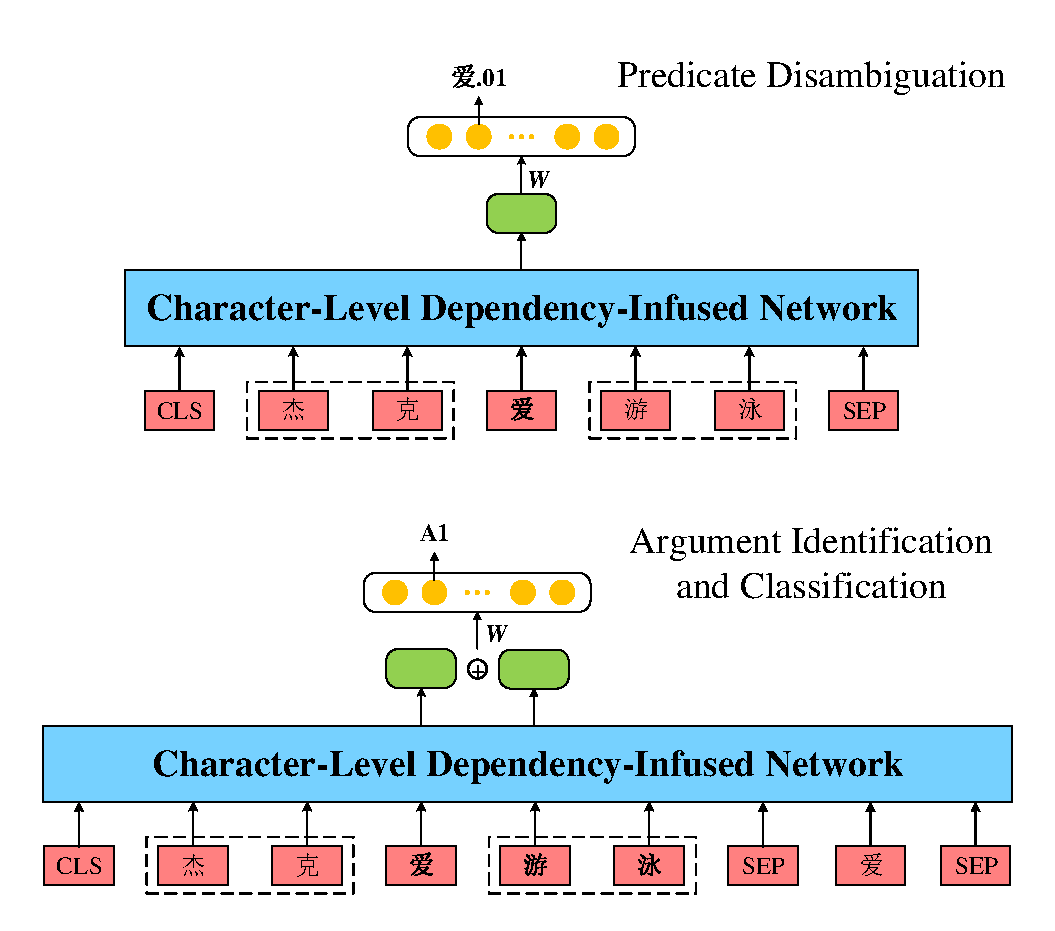
\includegraphics[width=0.85\textwidth]{figures/pipeline-srl-model.pdf}
	\bicaption[fig:pipeline-srl-model]{}{语义角色标注模型示意图}{Fig.$\!$}{Semantic role labeling model.}
\end{figure}

图\ref{fig:pipeline-srl-model}中下方模型为论元识别及分类模型,对于句中每个谓词,其首先将该谓词拼接到句子最后,用特殊符号“[SEP]”隔开。
也就是说对于每个谓词,该模型输入为:“[CLS] 句子 [SEP] 谓词 [SEP]”。
其中“[CLS]”和“[SEP]”都是BERT模型训练时使用的特殊符号,“[CLS]”作为句子开头符号,“[SEP]”则用于分开两个句子和表示句子结尾。
通过这种组合方式,句中其他词可以更好地获取当前谓词的信息。
之后通过本章提出的字级别依存关系强化网络获取每个词的向量表示,将当前谓词的向量和其他每一个词的向量分别进行拼接,然后通过一个前馈网络和softmax分类器预测当前谓词和其他词之间的语义关系:
\begin{equation}
    p(r|\bm{h}_p,\bm{h}_j) = \text{softmax}(\bm{W}[\bm{h}_p;\bm{h}_j)] + \bm{b})
\end{equation}
其中$\bm{h}_p$为当前谓词的表示向量,$\bm{h}_j$为句中第$j$个词的表示向量,$p(r|\bm{h}_p,\bm{h}_j)$表示第$j$个词与当前谓词间语义关系为$r$的概率。
在语义标签的集合中,有一个额外的“O”标签,用于表示当前词与谓词之间无关系。

\subsection{基于预训练模型的关系抽取模型}[Relation Extraction Model Based on Pre-trained Models]

关系抽取(Relation Extraction,简称RE)任务目的是预测句中给定的两个实体间的关系。
例如对于句子“我抬头看天”,给定两个实体分别为“我”和“头”,该任务需要预测二者的关系为Part-Whole,即部分与整体关系。

\begin{figure}[hbtp]
	\centering
	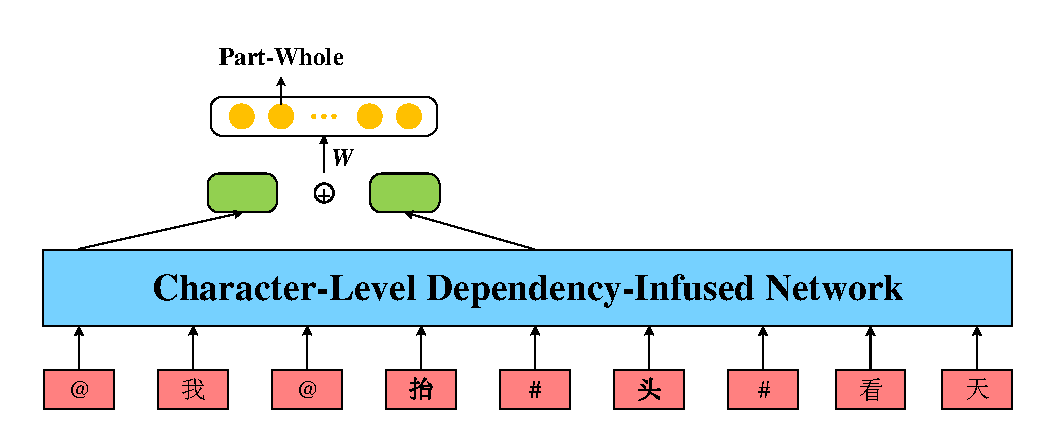
\includegraphics[width=0.85\textwidth]{figures/re-model.pdf}
	\bicaption[fig:re-model]{}{关系抽取模型示意图}{Fig.$\!$}{Relation Extraction model.}
\end{figure}

图\ref{fig:re-model}中给出了本章使用的关系抽取模型示意图。
具体来说,该模型首先在句中第一个实体的前后加上特殊符号“@”,然后在句中第二个实体的前后加上特殊符号“\#”。
经过这种修改,上述例句变为“@我@抬\#头\#看天”。
接着,将修改后的句子输入本章提出的字级别依存关系强化网络获取每个词的向量表示。
使用第一个实体前的“@”符号的向量作为其表示,使用第二个实体前的“\#”符号的向量作为其表示,然后拼接这两个向量,通过一个前馈网络和softmax分类器预测这两个实体之间的关系:
\begin{equation}
    p(r|\bm{h}_{@},\bm{h}_{\#}) = \text{softmax}(\bm{W}[\bm{h}_{@};\bm{h}_{\#})] + \bm{b})
\end{equation}
其中$\bm{h}_{@}$为第一个实体的表示向量,$\bm{h}_{\#}$为第二个实体的表示向量,$ p(r|\bm{h}_{@},\bm{h}_{\#})$表示两个实体间关系为$r$的概率。

\section{实验与分析}[Experiments and Analysis]

\subsection{实验设置}[Experimental Settings]

\subsection{语义角色标注实验结果}[]


\begin{table}[htpb]
    \bicaption[tbl:srl-result]{}{CoNLL 2009数据集上语义角色标注实验结果}{Table$\!$}{Semantic Role Labeling results on CoNLL-2009.}
    \vspace{0.5em}\centering\wuhao
    \begin{tabular}{lcccc}
        \toprule[1.5pt]
        模型 & & P & R & F1 \\
        \midrule[1pt]
        \multicolumn{4}{l}{\textit{w/o BERT}}  \\
        %\hline
        \citet{roth-lapata-2016-neural} & $\oslash$ & 83.2 & 75.9 & 79.4 \\
        \citet{marcheggiani-etal-2017-simple} & $\otimes$ & 83.4 & 79.1 & 81.2 \\
        \citet{he-etal-2018-syntax} & $\oslash$ & 84.2 & 81.5 & 82.8 \\
        \citet{li-etal-2018-unified} & $\oslash$ & 84.8 & 81.2 & 83.0 \\
        \citet{he-etal-2019-syntax} & $\odot$ & 84.6 & 84.5 & 84.6 \\
        \citet{munir-etal-2021-adaptive} & $\oslash$ & 84.7 & 85.1 & 84.9 \\
        \citet{xia-etal-2019-syntax} & $\oslash$ & 84.6 & 85.7 & 85.1 \\
        \hline
        \multicolumn{4}{l}{\textit{w/ BERT}}  \\
        %\hline
        \citet{he-etal-2019-syntax} & $\odot$ & 86.2 & 86.7 & 86.4 \\
        \citet{xia-etal-2019-syntax} & $\oslash$ & 88.0 & 89.1 & 88.5 \\
        \citet{li-etal-2020-high} & $\otimes$ & -	& - & 88.7 \\
        Baseline & $\otimes$ & 88.2 & 88.3 & 88.2 \\
        Word-Level GCN & $\oslash$ & 88.6 & 88.5 & 88.5 \\
        Word-Level GCN & $\odot$ & 90.8 & 90.3 & 90.5  \\
        Ours & $\oslash$ & 89.2 & 88.5 & 88.9 \\
        Ours & $\odot$ & 91.9 & 91.8 & 91.9  \\
        \hline
        \multicolumn{4}{l}{\textit{w/ RoBERTa}}  \\
        %\hline
        Baseline & $\otimes$ & 88.6 & 88.1 & 88.4 \\
        Word-Level GCN &$\oslash$ & 88.7 & 88.6 & 88.6 \\
        Word-Level GCN &$\odot$ & 90.3 & 90.5 & 90.4 \\
        Ours &$\oslash$ & 88.9 & 89.1 & 89.0 \\
        Ours &$\odot$ & 92.2 & 92.0 & 92.1 \\
        \bottomrule[1.5pt]
    \end{tabular}
\end{table}



\subsection{关系抽取实验结果}


\begin{table}[htpb]
    \bicaption[tbl:srl-result]{}{FinRE和SanWen数据集上关系抽取实验结果}{Table$\!$}{Relation Extraction results on FinRE and SanWen.}
    \vspace{0.5em}\centering\wuhao
    \begin{tabular}{lc}
        \toprule[1.5pt]
        模型 & F1 \\
        \midrule[1pt]
        \multicolumn{2}{c}{SanWen} \\
        \hline
        \citet{xu-etal-2020-chinese} & 57.43 \\
        \citet{zhang-yu-2020-chinese} & 63.13 \\
        \citet{li-etal-2019-chinese} & 65.61 \\
        BERT & 76.75 \\
        BERT + SDG & \bf 77.73 \\
        \hline
        \multicolumn{2}{c}{FinRE} \\
        \hline
        Li et al. & 49.26 \\
        BERT & 56.82 \\
        BERT + SDG & \bf 57.26 \\
        \bottomrule[1.5pt]
    \end{tabular}
\end{table}


\section{本章小结}[Conclusions]


% Local Variables:
% TeX-master: "../thesis"
% TeX-engine: xetex
% End: